\section{Scelte implementative}
\label{cap:implementation-choices}

\subsection{Rappresentazione dei grafi}
\label{sub:graph-representation}

Gli algoritmi di questo homework operano su grafi pesati completamente connessi e non diretti. Ha quindi senso rappresentare ogni grafo con una Matrice di Adiacenza, dato che i grafi sono completi. In questa relazione useremo in maniera ambivalente i termini \textit{Matrice di Adiacenza} e \textit{Matrice delle distanze}, poiché i grafi sono pesati.

\noindent I dataset contenenti i grafi di input sono in formato standard \textbf{TSPLIB } e riportano le coordinate 2D dei nodi del grafo in due possibili formati:

\begin{itemize}
    \item \textbf{EUC\_2D}: le coordinate rappresentano la posizione nello spazio euclideo a 2 dimensioni. È dunque richiesto il calcolo della distanza euclidea tra ogni nodo, con il valore arrotondato al numero intero più vicino;
    \item \textbf{GEO}: le coordinate rappresentano la latidudine e la longitudine di ogni punto. Il calcolo della distanza tra due punti in questo caso è più complesso, e richiede una conversione preliminari in radianti. Tale conversione avviene nel costruttore della classe \codeinline{point\_geo}, definita nel file \codeinline{Shared/point.h}.
\end{itemize}

La formula usata per il calcolo della distanza euclidea è mostrata nel listing \ref{listing:euclidean-distance}, mentre la formula usata per calcolare la distanza geodesica è illustrata nel listing \ref{listing:geodesic-distance}. Si noti che tali distanze non sono esatte, ma seguono i criteri di approssimazione a distanze intere definiti nella specifica dell'homework.

\begin{listing}[!ht]
\begin{minted}{c++}
// Shared/euclidean_distance.h

int euclidean_distance(const point::point_2D& i,
                      const point::point_2D& j) noexcept {
    const auto& [x_i, y_i] = i;
    const auto& [x_j, y_j] = j;

    const double x = x_i - x_j;
    const double y = y_i - y_j;

    // distanza euclidea tra i punti i e j
    const double distance = std::sqrt(std::pow(x, 2) + std::pow(y, 2));

    // arrotonda al valore intero più vicino
    return static_cast<int>(std::round(distance));
}
\end{minted}
\caption{Funzione per il calcolo della distanza Euclidea approssimata tra due punti.}
\label{listing:euclidean-distance}
\end{listing}

\begin{listing}[!ht]
\begin{minted}{c++}
// Shared/geodesic_distance.h

int geodesic_distance(const point::point_geo& i,
                      const point::point_geo& j) noexcept {
    // raggio equatoriale approssimato della terra, in km
    constexpr double RRR = 6378.388;

    const auto& [lat_i, long_i] = i;
    const auto& [lat_j, long_j] = j;

    const double q1 = std::cos(long_i - long_j);
    const double q2 = std::cos(lat_i - lat_j);
    const double q3 = std::cos(lat_i + lat_j);

    // distanza geodesica tra i punti i e j, che sono stati convertiti
    // precedentemente in radianti
    const double distance = RRR *
        std::acos(0.5 * ((1.0 + q1) * q2 - (1.0 - q1) * q3)) + 1.0;

    // ritorna la parte intera della distanza geodesica
    return static_cast<int>(std::trunc(distance));
}
\end{minted}
\caption{Funzione per il calcolo della distanza geodesica approssimata tra due punti.}
\label{listing:geodesic-distance}
\end{listing}

\noindent I risultati del calcolo delle distanze (\textit{EUC\_2D} o \textit{GEO} a seconda del dataset di input) sono inseriti nella posizione corrispondente della Matrice delle Distanze.
Una volta calcolate le distanze, le coordinate originali non sono mantenute: non sono infatti necessarie ai fini della rappresentazione del grafo e del calcolo della soluzione di TSP.
Nella figura \ref{fig:distancematrix-example} è possbile vedere un esempio di una conversione di un grafo di esempio rappresentato da cordinate EUC\_2D nella sua matrice delle distanze.

\begin{figure}[h]
	\centering
	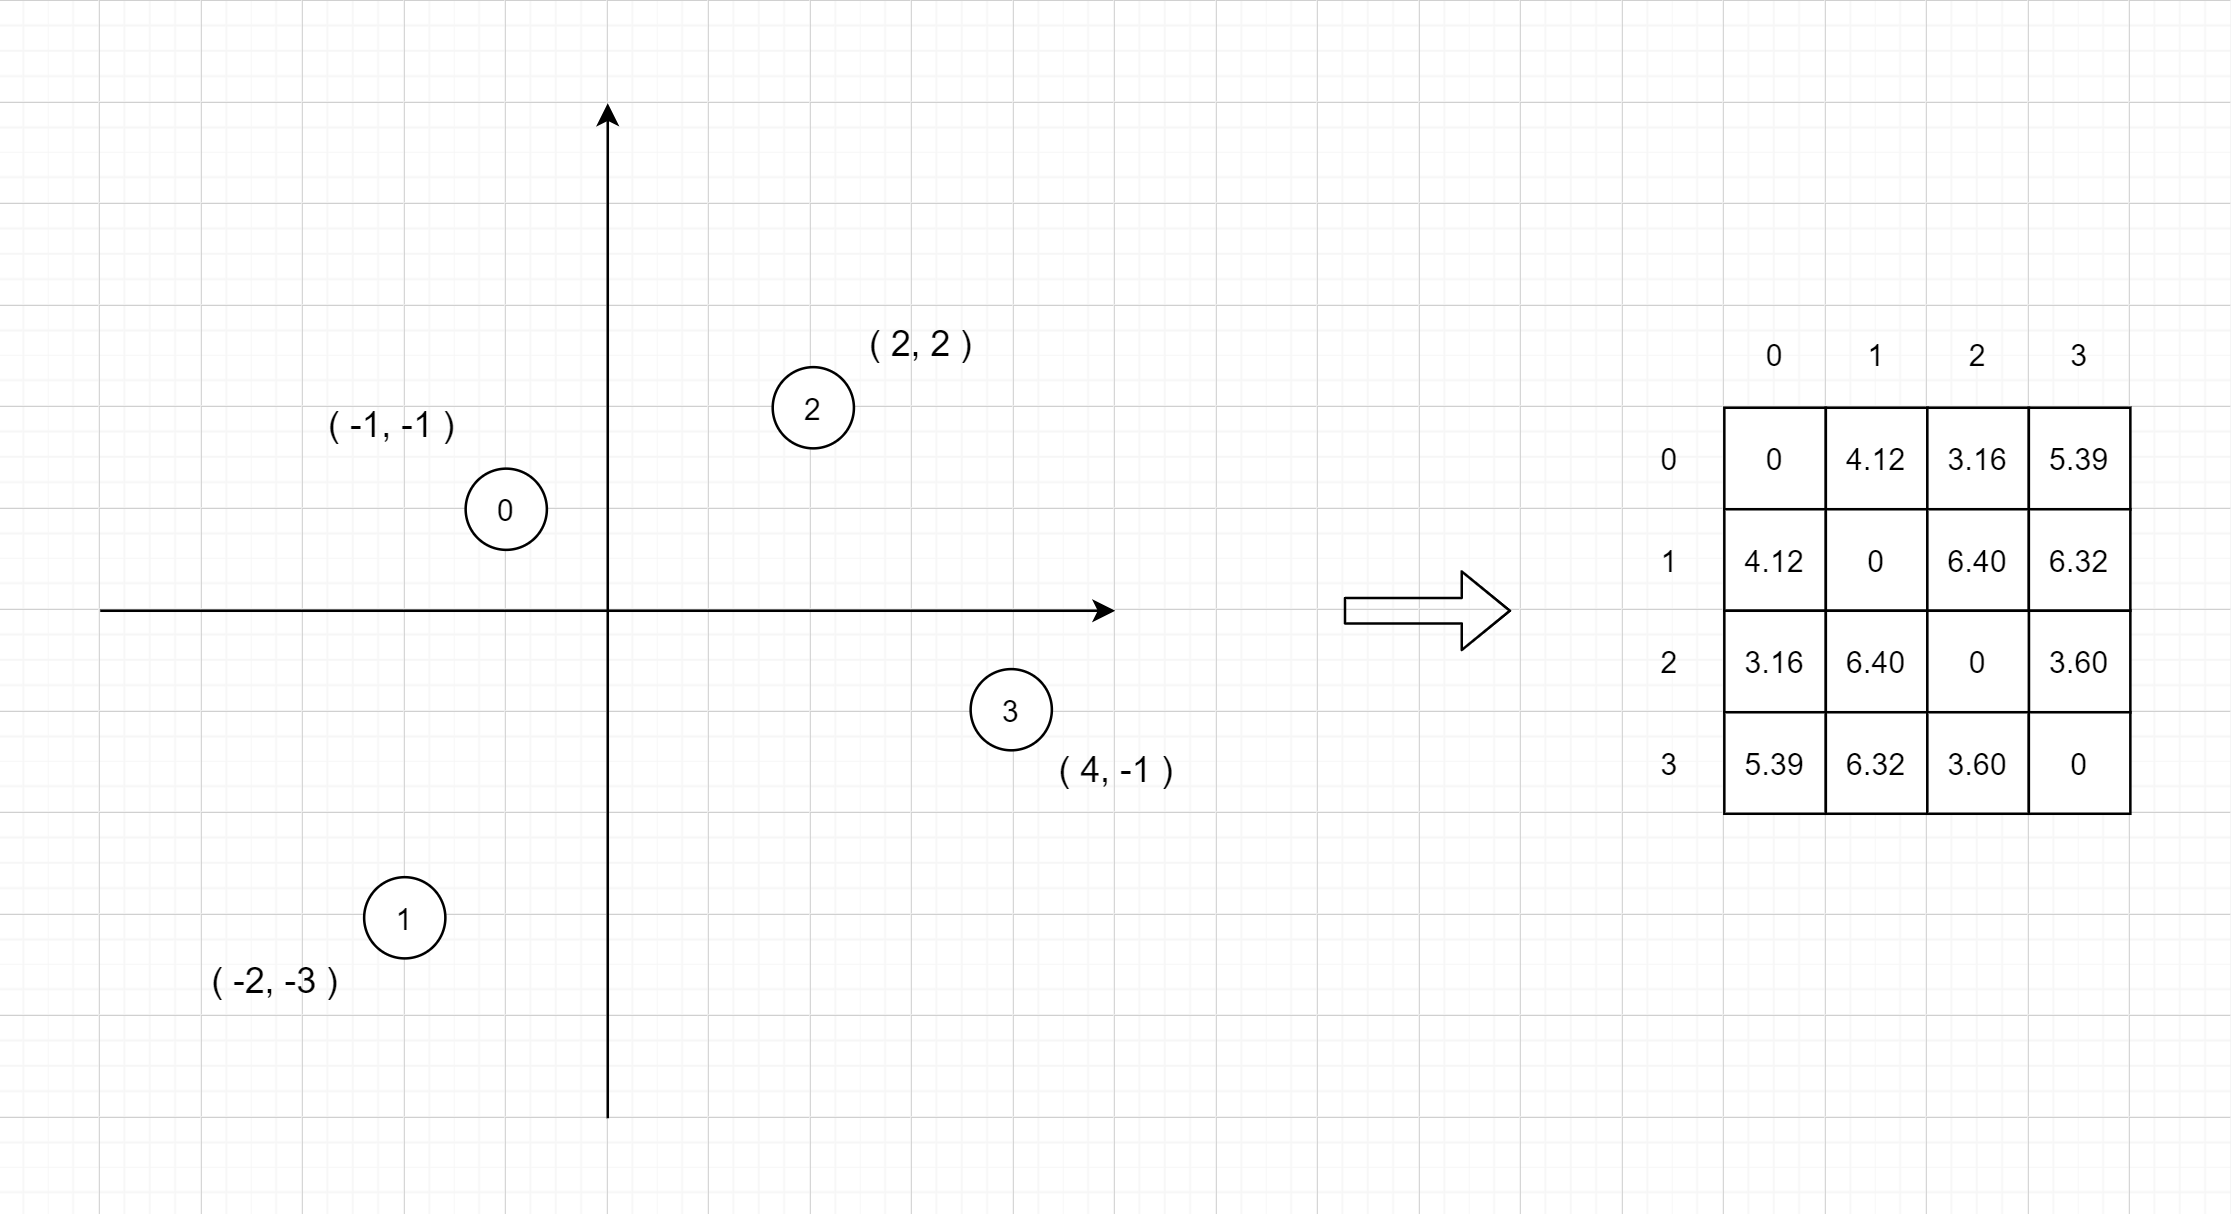
\includegraphics[width=0.9\textwidth]{./images/Distance Matrix.png}
	\caption{Grafo di esempio rappresentato con Matrice delle distanze}
	\label{fig:distancematrix-example}
\end{figure}

\noindent Come nel precedente homework, per semplificare la logica di indicizzazione dei nodi del grafo, la label dei nodi (originariamente numerata da $1$ a $n$) è decrementata di 1, quindi i nodi sono rappresentati dall'intervallo numerico $[0, n-1]$.

\noindent La classe che rappresenta la Matrice delle Distanze dei grafi è definita in \codeinline{DistanceMatrix.h} nella cartella \textit{Shared}.

\begin{listing}[!ht]
\begin{minted}{c++}
std::vector<T> data;

// mappa la coppia di indici (row, column) della matrice in un indice per
// il vettore 1-dimensionale data. (Indicizzazione fisica)
[[nodiscard]] size_t get_index(size_t row, size_t column) const noexcept {
    return row * n_vertexes + column;
}

// valore della distanza tra i nodi (i, j). (Indicizzazione virtuale)
[[nodiscard]] T& at(size_t i, size_t j) noexcept {
    return data.at(get_index(i, j));
}
\end{minted}
\caption{Indicizzazione virtuale e fisica della classe \codeinline{DistanceMatrix.h}.}
\label{listing:virtual-physica-addressing}
\end{listing}

\paragraph{Ottimizzazioni}\mbox{} \\

\noindent Poichè i grafi in esame sono non diretti ($\forall i,j \in V$, $c(i,j) = c(j,i)$), la Matrice delle Distanze è una matrice simmetrica con tutte le entry della diagonale principale pari a 0 (in quanto ogni vertice dista 0 da se stesso).
Abbiamo quindi calcolato le distanze \textit{pair-wise} solo per la parte triangolare superiore della matrice, per poi copiarle in maniera trasposta nella parte triangolare inferiore. Questo ci ha permesso quindi di evitare di calcolare le stesse distanze più volte. \\

\noindent La matrice è rappresentata da un singolo \codeinline{std::vector}. Questo dà la garanzia che ogni riga della matrice sia definita in sezioni contigue di memoria, riduce l'overhead rispetto ad un approccio \codeinline{std::vector<std::vector>}, e, nonostante la logica di indicizzazione sia un po' più complessa (l'indicizzazione virtuale è a due dimensioni, quella fisica è ad una sola dimensione), il cache behaviour della classe è migliore, dando risultati mediamente più performanti. Si veda il listing \ref{listing:virtual-physica-addressing} per osservare la relazione tra indirizzamente fisico e virtuale nella classe \codeinline{DistanceMatrix.h}.

\begin{listing}[!ht]
\begin{minted}{c++}
int main(int argc, char** argv) {
    if (argc != 2) {
        std::cerr << "1 argument required: filename" << std::endl;
        exit(0);
    }

    const char* filename = argv[1];

    // legge il grafo completo non diretto dal file di input
    auto point_reader(read_file(filename));

    // crea la matrice di distanza, usando le distanze euclidea o geodesica a seconda
    // del tipo di input
    DistanceMatrix<int> distance_matrix = point_reader->create_distance_matrix();

    // calcola il peso della soluzione TSP individuata dall'algoritmo
    const auto total_weight = ...;

    // stampa la soluzione trovata
    std::cout << std::fixed << total_weight << std::endl;
}
\end{minted}
\caption{Scheletro comune ad ogni file \codeinline{main.cpp} del progetto.}
\label{listing:main-cpp}
\end{listing}

\subsection{Lettura del Grafo}

\noindent Il file \codeinline{main.cpp} ha la stessa struttura per ogni algoritmo, si veda il listing \ref{listing:main-cpp}. Ad alto livello, le operazioni svolte sono:

\begin{enumerate}
    \item Lettura del file di input: il file di input viene parsato da \codeinline{read\_file.h}, e vengono lette solo le informazioni più importanti, ovvero:

    \begin{itemize}
        \item dimensione del grafo;
        \item tipo di distanza (\textit{EUC\_2D} o \textit{GEO});
        \item coordinate del grafo.
    \end{itemize}

    \noindent Abbiamo usato la libreria di file streaming nativa di C++ (\codeinline{fstream}). Abbiamo rappresentato il tipo di distanza con l'\mintinline{c++}{enum} \codeinline{EdgeWeightType.h}, per la quale abbiamo definito l'operatore di lettura \mintinline{c++}{std::istream& operator>>}.

    \item I punti definiti dopo la riga \textit{NODE\_COORD\_SECTION} dei dataset di input sono letti con un'istanza polimorfica di \codeinline{PointReader.h}, che interpreta le coordinate in maniera diversa a seconda del valore assunto dall'enumerazione \codeinline{EdgeWeightType}, ovvero a seconda del tipo di distanza del file. Naturalmente, la sottoclasse \codeinline{EuclideanPointReader.h} usa la distanza Euclidea, mentre \codeinline{GeodesicPointReader.h} usa quella geodesica. Le classi dei punti letti in input sono definiti in \codeinline{point.h} (\codeinline{point\_2D} per le coordinate euclidee, \codeinline{point\_geo} per le coordinate geografiche), e per ognuno di essi è stato definito l'operatore di lettura \mintinline{c++}{std::istream& operator>>} adeguato. Questo ci ha permesso di non avere duplicazione di codice per gestire tipi diversi di punti in input. \\

    \noindent La label dei nodi è decrementata di 1 in questa fase di lettura.

    \item Una volta letti i nodi, viene creata la matrice delle distanze applicando il \textit{Template Method Pattern}, usando la nozione di distanza definita dalle sottoclassi di \codeinline{PointReader.h}. Il metodo concreto \codeinline{distance(i, j)} delle sottoclassi è usato nel costruttore di \codeinline{DistanceMatrix} come \textit{higher-order function}. Si veda il listing \ref{listing:point-reader}.
\end{enumerate}

Tutti i file citati qui sopra sono nella cartella \textit{Shared} del progetto consegnato.

\begin{listing}[!ht]
\begin{minted}{c++}
class PointReader {
protected:
  std::fstream& file;
  size_t dimension;

  // calcola la distanza tra i punti i e j
  virtual int distance(size_t i, size_t j) const = 0;

public:
  PointReader(std::fstream& file, size_t dimension) :
    file(file), dimension(dimension) { }

  virtual ~PointReader() = default;

  // consuma la lista di coordinate dal file di input
  virtual void read() = 0;

  // crea la matrice delle distanze a partire dai punti letti. Usa il metodo distance
  // implementato dalle sotto classi come funzione higher-order
  DistanceMatrix<int> create_distance_matrix() {
    using namespace std::placeholders;
    auto distance_fun(std::bind(&PointReader::distance, this, _1, _2));

    return DistanceMatrix<int>(dimension, distance_fun);
  }
};
\end{minted}
\caption{Definizione parziale di \codeinline{PointReader.h} che evidenza la creazione della matrice delle distanze del grafo letto.}
\label{listing:point-reader}
\end{listing}

\subsection{Strutture Dati comuni}

Tutte le strutture dati elencate di seguito sono definite nella cartella \textit{Shared}.
Ove possibile, per la nomenclatura dei metodi abbiamo cercato di seguire lo stesso standard dei container STL di C++.
Inoltre, le strutture dati usate sono sempre pre-allocate in memoria quando possibile, evitando rehashing e riallocazioni dispendiose. Questo significa che la maggior parte delle operazioni indicate con \complexityConstant{} ammortizzato siano in realtà totalmente costanti nella pratica. \\

\noindent Le strutture dati relative alle Heap e alle code di priorità necessarie per l'algoritmo di Prim sono già state ampiamente documentate nell'homework 1.

\subsection{Rappresentazioni dei grafi alternative}

\noindent L'algoritmo di $2$-approssimazione basato sul calcolo del Minimum Spanning Tree fa uso di due rappresentazioni diverse per i grafi.
\codeinline{DistanceMatrix.h} è usato per leggere il grafo in input ed eseguirne l'algoritmo di Prim (che è stato adattato dal precedente homework). \codeinline{AdjacencyMapGraph.h}, che contiene un subset definite per la Mappa di Adiacenza definita nel precedente homework, è invece usata per rappresentare il Minimum Spanning Tree all'interno di \codeinline{DFS.h}, che lo scorre per generare il vettore della visita \textit{Preorder}. Questa scelta è dovuta al fatto che l'MST non è completo come il grafo di input, e anzi contiene solo $n - 1$ archi. Una Matrice di adiacenza è quindi inutilmente costosa in termini di spazio in questo caso.

\newpage
\subsection{Rappresentazione dei circuiti parziali di Held \& Karp}

L'algoritmo Held-Karp richiede esplicitamente l'uso di due vettori:
\begin{itemize}
    \item $d[v,S]$ è il peso del cammino minimo che parte da 0 e termina in v, visitando tutti i nodi in S;
    \item $\pi[v,S]$ è il predecessore di v nel cammino minimo definito come sopra.
\end{itemize}

\noindent Poiché l'homework richiede la restituizione del peso del cammino Hamiltoniano inferiore e non il cammino stesso, abbiamo omesso il vettore $\pi[v,S]$. \\

Abbiamo rappresentato la tabella $d[v,S]$ usata dall'algoritmo di programmazione dinamica come una mappa chiave-valore, dove:

\begin{itemize}
    \item la chiave è una coppia $(S, v)$;
    \item il valore è il peso del cammino minimo che parte dal nodo 0 e termina in $v$, visitando tutti i nodi in $S$.
\end{itemize}

\noindent Il tipo della mappa è:

\begin{center}
    \mintinline{c++}{std::unordered_map<std::pair<decltype(S), size_t>, int>}
\end{center}

\noindent Poiché le distanze euclidea e geodesica sono approssimate a valori interi, il tipo del valore della mappa è \mintinline{c++}{int}.
Per rappresentare il set di nodi $S$ abbiamo studiato 3 possibili soluzioni.

\subsubsection{Rappresentazione del circuito parziale S}
\label{held-karp-S-repr}

Di seguito sono presentate le 3 possibili soluzioni che abbiamo individuato per rappresentare il circuito parziale $S$ dell'algoritmo di Held \& Karp. Ricordiamo che $S$ fa parte della chiave di una \mintinline{c++}{std::unordered_map}, quindi deve esistere un metodo che definisca l'hash di $S$.

\paragraph{Unordered Set}\mbox{}\\

\noindent La soluzione più semplice per rappresentare un insieme di vertici senza ripetizioni è usare la struttura dati \mintinline{c++}{std::unordered_set}. La tabella \ref{tab:pro-cons-unordered-set} evidenzia i pro e i contro di questo approccio. Osserviamo in particolare che lo spazio occupato per rappresentare un circuito parziale può essere compattato, il che può essere d'aiuto, visto che Held \& Karp ha un'occupazione spaziale esponenziale sulla taglia dell'input. \\

\noindent Notiamo inoltre che la libreria standard non definisce alcun metodo \\ \mintinline{c++}{std::hash<std::unordered_set<T>>}, quindi è spettata a noi la definizione della \textit{hash function} per questa struttura dati. Si veda la sezione \ref{hashing} per ulteriori informazioni. TODO: aggiungere questa sezione.

\begin{table}
  \centering
    \begin{tabular}{|c | c|}
    \hline
    \textbf{PRO} & \textbf{CONTRO} \\ [0.5ex]
    \hline\hline
    Offerta dalla libreria standard di C++ & Ha un'occupazione spaziale lineare\\
    \hline
    Rende evidente la non esistenza di nodi ripetuti & La libreria standard non ne definisce l'hash \\
    \hline
    Facile da usare &  \\
    \hline
  \end{tabular}
    \caption{Analisi dei pro e contro di std::unordered\_set.}
    \label{tab:pro-cons-unordered-set}
\end{table}

\noindent Il tipo della mappa in questo caso è:

\begin{center}
    \mintinline{c++}{std::unordered_map<std::pair<std::unordered_set<size_t>, size_t>, int>}
\end{center}

\paragraph{Tecnica bit masking}\mbox{}\\

\begin{table}
  \centering
    \begin{tabular}{|c | c|}
    \hline
    \textbf{PRO} & \textbf{CONTRO} \\ [0.5ex]
    \hline\hline
    Massima compattezza spaziale & Complesso da usare \\
    \hline
    Rende evidente la non esistenza di nodi ripetuti & Supporta solo architetture a 64 bit \\
    \hline
    La libreria standard ne definisce l'hash & Usabile solo per grafi con $n \leq 63$ \\
    \hline
  \end{tabular}
    \caption{Analisi dei pro e contro della tecnica bit masking per numeri interi senza segno.}
    \label{tab:pro-cons-bit-masking}
\end{table}

\noindent \textbf{Premessa}: per questo metodo, abbiamo assunto che i programmi saranno eseguiti solo su architetture a 64 bit. I grafi con più di 63 nodi non possono essere rappresentati con questo metodo. \\

\noindent Una soluzione migliore per rappresentare in maniera estremamente compatta il set di nodi visitati $S$ è usare un singolo numero intero senza segno a 64 bit. In questo caso, ogni bit a 1 rappresenta la presenza di un vertice $i$ nell'insieme $S$.
Se il bit all'$i$-esima posizione nel numero vale 1, allora il vertice $i \in S$, se il bit vale invece 0 allora $i \notin S$. La tabella \ref{tab:pro-cons-bit-masking} evidenzia i pro e i contro di questo approccio. \\

\noindent Nel nostro linguaggio, il tipo necessario a definire numeri interi senza segno a 64 bit è \\
\mintinline{c++}{unsigned long long}. Si consideri l'esempio in figura \ref{fig:bitmasking-example} per vedere come è possibile rappresentare $S$ in questo modo.

\begin{figure}[h]
	\centering
	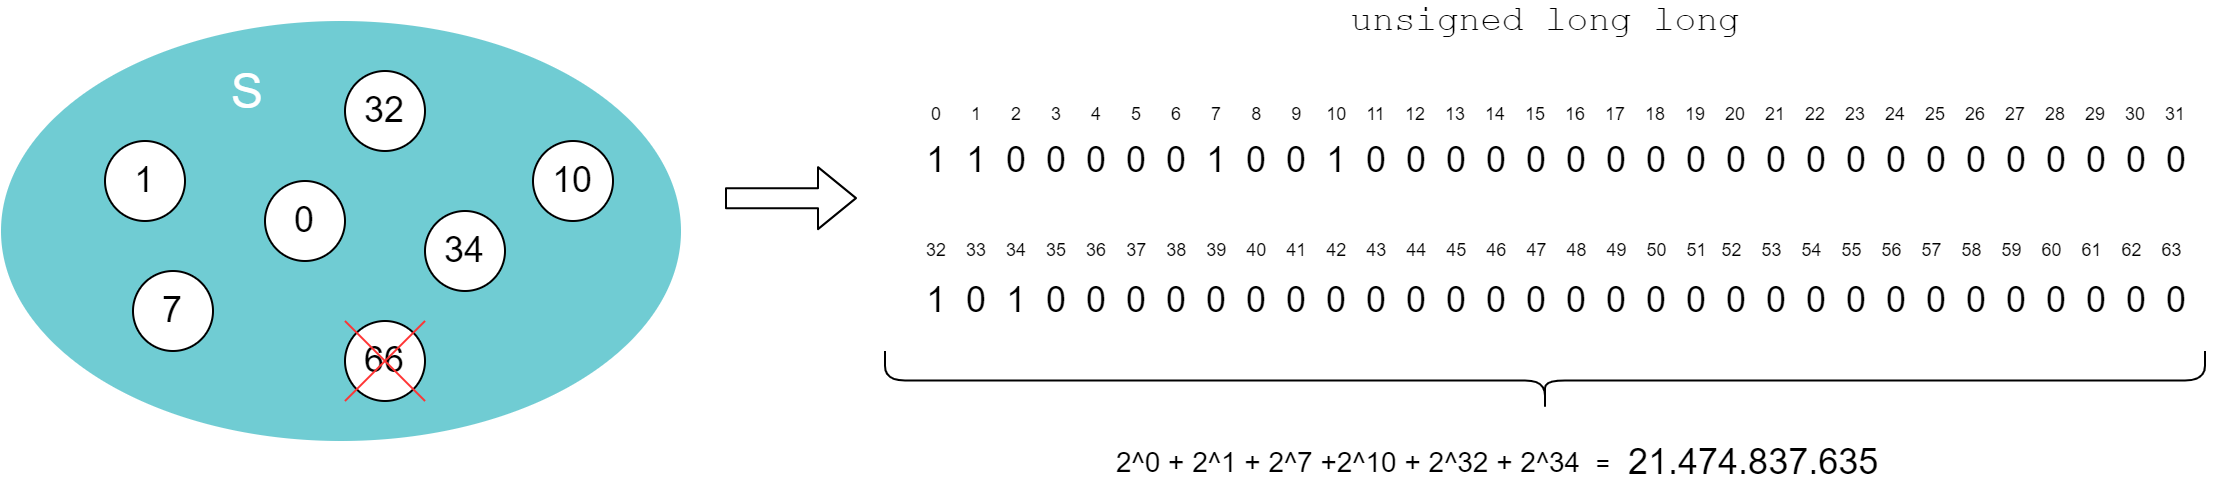
\includegraphics[width=0.9\textwidth]{./images/BitMasking Example.png}
	\caption{Rappresentazione di S tramite BitMasking}
	\label{fig:bitmasking-example}
\end{figure}

\noindent Con questa rappresentazione chiamata \textit{bit masking}, eliminazione, aggiunta e verifica della presenza di vertici in $S$ sono implementate sfruttando operazioni $AND$, $OR$, $XOR$ bit-a-bit e bit-shifting.
Poiché questo tipo di operazioni si traduce in una singola istruzione Assembly, manipolare $S$ tramite bit-masking è estremamente performante sia dal punto di vista temporale che spaziale. \\

\noindent Un limite di tale struttura è l'impossibilità di poter rappresentare un set $S$ che contiene più di 64 nodi, come è possibile vedere nell'esempio della figura \ref{fig:bitmasking-example} dove il vertice 66 non può essere rappresentato in questo modo. Il limite di rappresentazione di $S$ in realtà scende a 63 nodi per via delle operazioni di bit-shift necessarie a manipolare il circuito parziale.

\noindent Il tipo della mappa in questo caso è:

\begin{center}
    \mintinline{c++}{std::unordered_map<std::pair<unsigned long long, size_t>, int>}
\end{center}

\paragraph{Struttura dati ad-hoc: DynamicBitMasking}\mbox{} \\

Per superare il limite della rappresentazione tramite BitMasking per più di 63 nodi si è pensato di estendere l'idea del BitMasking non più ad un solo numero, ma a più numeri. In questo modo se il set S può raggiungere cardinalità più grandi di 64 nodi è possibile rappresentarlo con più di un numero, dove il primo numero rappresenta i primi 64 nodi, il secondo i successivi 64 nodi e così via. Per fare questo abbiamo dichiarato un'apposita classe chiamata \textit{DynamicBitMasking} che tramite un \textit{std::vector} di \textit{unsigned long long} è in grado di rappresentare qualunque set S. In questo modo, data una posizione di un bit $i$, è sufficiente ricavarsi l'indice del vettore dove risiede il numero che contiene il bit $i$ (tramite la divisione intera di $i$ con 64) e la posizione del bit all'interno del numero (tramite il resto della divisione di $i$ con 64). Nell'esempio raffigurato in figura \ref{fig:DynamicBitMasking-example} è possibile vedere come lo stesso set S visto nell'esempio precedente ora possa essere rappresentato tramite questa nuova struttura dati.

\begin{figure}[h]
	\centering
	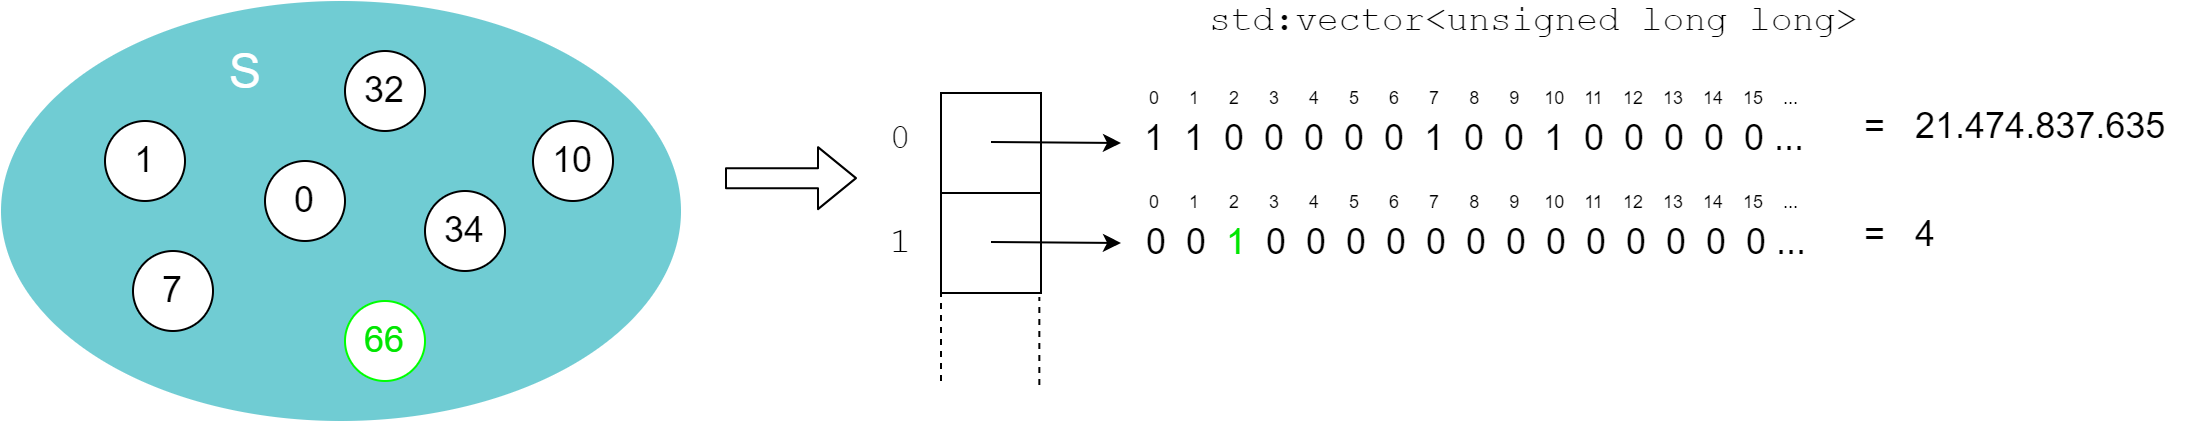
\includegraphics[width=0.9\textwidth]{./images/BitMaskingExtended Example.png}
	\caption{Rappresentazione di S tramite DynamicBitMasking}
	\label{fig:DynamicBitMasking-example}
\end{figure}

\paragraph{Confronto tra unordered\_set, BitMasking ed DynamicBitMasking}
In questo paragrafo vogliamo mettere a confronto le performance in termini di complessità spaziali e temporali delle 3 soluzioni proposte. Nella grafico riportato in figura \ref{fig:UnorderedvsDynamicBitMasking} abbiamo voluto mettere a confronto i tempi esatti dell'esecuzione delle 3 varianti proposte con grafi a 14, 16 e 22 nodi.

\begin{figure}[h]
	\centering
	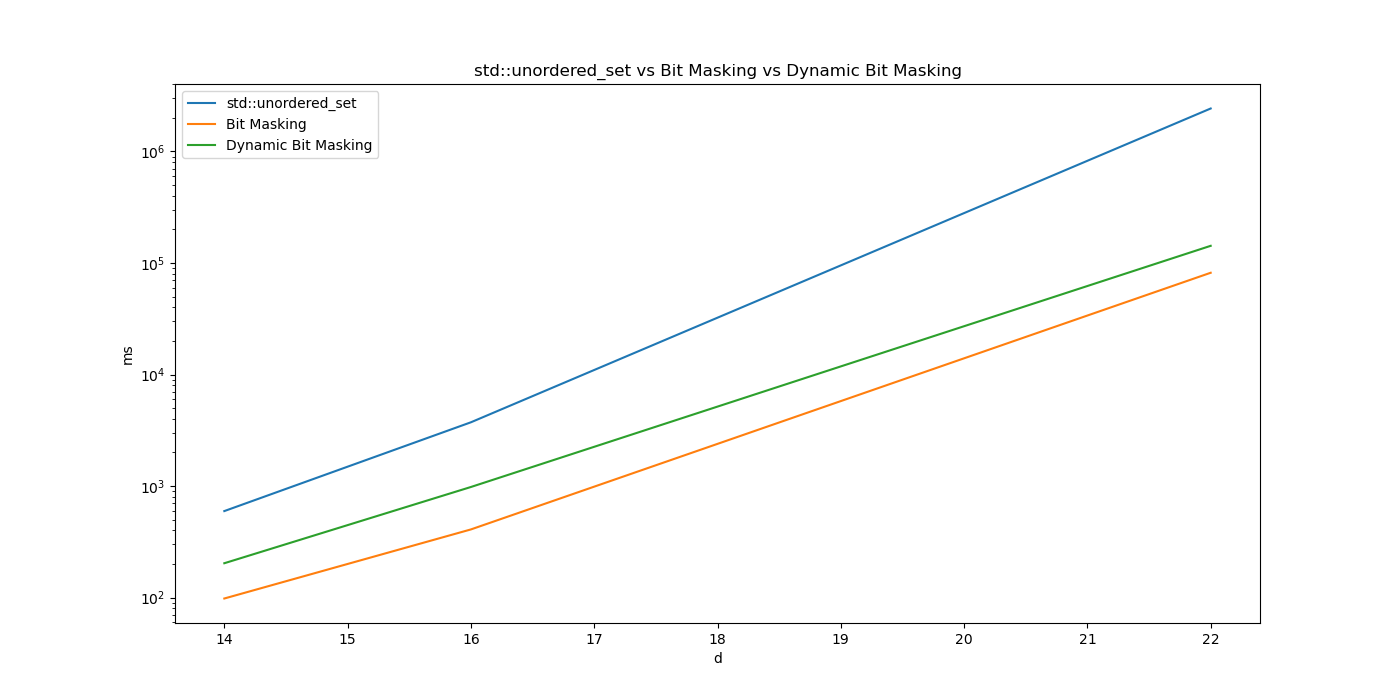
\includegraphics[width=1\textwidth]{./images/unorderedSet vs BitMasking.png}
	\caption{Confronto dei tempi di esecuzione di Held-Karp al crescere del numero di nodi usando unordered\_set, BitMasking ed DynamicBitMasking. I dataset usati per il confronto sono \codeinline{burma14}, \codeinline{ulysses16} e \codeinline{ulysses22}.}
	\label{fig:UnorderedvsDynamicBitMasking}
\end{figure}

Come è possibili notare, l'implementazione più veloce risulta essere il BitMasking a 64 bit, in quanto utilizzando un solo numero per rappresentare i nodi in S, l'overhead è inferiore rispetto alle operazioni da svolgere per DynamicBitMasking che deve calcolarsi la posizione del bit all'interno di più numeri. In ogni caso DynamicBitMasking è in grado di svolgere egregiamente il suo lavoro, avendo un tempo di esecuzione molto inferiore rispetto alla soluzione semplice con unordered\_set.

Visti i seguenti risultati si è quindi deciso di utilizzare la versione BitMasking a 64 bit per i grafi con meno di 64 nodi e la versione DynamicBitMasking per i grafi con più di 64 nodi.

\subsection{Timeout}

\noindent L'algoritmo di Held-Karp ha complessità temporale \complexityHeldKarpTime{}, quindi i tempi di esecuzione \textit{esplodono} anche solo per grafi con poche decine di nodi. Come richiesto dall'homework, all'algoritmo di Held-Karp è assegnato un timeout di esecuzione $T$. Abbiamo fissato il valore di $T$ a 2 minuti, per mantenere la RAM occupata sotto controllo (anche la complessità spaziale dell'algoritmo è esponenziale).\\

\noindent La nostra implementazione di Held-Karp, quindi:

\begin{enumerate}
    \item Ritorna la soluzione esatta se i suoi tempi di esecuzione sono inferiori a 2 minuti, senza aspettare lo scadere del timeout;
    \item Se invece il timeout scade, termina preventivamente la ricorsione e ritorna la migliore soluzione trovata fino a quel momento. A seconda della profondità del call-stack ricorsivo, la soluzione potrebbe essere ritornata qualche secondo dopo lo scadere del timeout.
\end{enumerate}

\noindent C++17 non fornisce soluzione \textit{out-of-the-box} ad alto livello per eseguire funzioni con un limite di tempo. Abbiamo quindi implementato un meccanismo di questo tipo in \codeinline{Shared/timeout.h}, il cui funzionamento ad alto livello è il seguente:

\begin{itemize}
    \item Il thread principale crea un \textit{worker thread} incaricandolo di eseguire Held-Karp sul grafo letto in input. Fa quindi partire il timeout e resta in attesa del risultato del worker thread. Tale risultato sarà disponibile da un \codeinline{std::future}.
    \item Se il worker thread termina prima dello scadere del timeout, il thread principale è immediatamente sbloccato e il risultato della funzione (restituito da \codeinline{std::future::get()}) è ritornato al chiamante.
    \item Se il timeout scade e il worker thread non ha ancora terminato l'esecuzione, il thread principale gli notifica di terminare l'esecuzione il prima possibile. Tale notifica avviene forzando la conclusione di una \codeinline{std::promise} creata dal main thread e data in input alla funzione eseguita incapsulata nella classe \codeinline{timeout\_signal}.
    \item Quando la funzione eseguita si accorge che il tempo a disposizione è scaduto, interrompe la ricorsione e ritorna la migliore soluzione individuata fino a quel momento al chiamante.
\end{itemize}
